\documentclass[letterpaper]{article}

\usepackage{natbib,alifeconf,amsmath,amssymb,amsfonts}  %% The order is important
\usepackage{graphicx}
\usepackage{textcomp}
\usepackage{relsize}
%\usepackage{geometry}
%\usepackage{lipsum}
\usepackage{algpseudocode}
\renewcommand{\algorithmicrequire}{\textbf{Input:}}
\renewcommand{\algorithmicensure}{\textbf{Output:}}
\usepackage{array}
%\usepackage{caption}
%\usepackage[caption=false,font=footnotesize]{subfig}
%\usepackage{fixltx2e}
\usepackage{float}
\usepackage{url}
%\usepackage{becs}
\usepackage{listings}
\lstset{%
  basicstyle=\normalsize,
  numbers=left,
  numberstyle=\normalsize,
  stepnumber=1,
  xleftmargin=2em
}
%\usepackage{color}
\def\BibTeX{{\rm B\kern-.05em{\sc i\kern-.025em b}\kern-.08em
T\kern-.1667em\lower.7ex\hbox{E}\kern-.125emX}}
\interdisplaylinepenalty=2500
\newtheorem{definition}{Definition}
\newtheorem{exampleb}{Example}
\newcommand{\subsubsubsection}[1]{\medskip\par\textit{#1:}}
\newcommand{\card}[1]{\vert{#1}\vert}
\newcommand{\magn}[1]{\vert{#1}\vert}
\hyphenation{op-tical net-works semi-conduc-tor}
\usepackage{xcolor}
\usepackage{standalone}


% *****************
%  Requirements:
% *****************
%
% - All pages sized consistently at 8.5 x 11 inches (US letter size).
% - PDF length <= 8 pages for full papers, <=2 pages for extended
%    abstracts.
% - Abstract length <= 250 words.
% - No visible crop marks.
% - Images at no greater than 300 dpi, scaled at 100%.
% - Embedded open type fonts only.
% - All layers flattened.
% - No attachments.
% - All desired links active in the files.

% Note that the PDF file must not exceed 5 MB if it is to be indexed
% by Google Scholar. Additional information about Google Scholar
% can be found here:
% http://www.google.com/intl/en/scholar/inclusion.html.


% If your system does not generate letter format documents by default,
% you can use the following workflow:
% latex example
% bibtex example
% latex example ; latex example
% dvips -o example.ps -t letterSize example.dvi
% ps2pdf example.ps example.pdf


% For pdflatex users:
% The alifeconf style file loads the "graphicx" package, and
% this may lead some users of pdflatex to experience problems.
% These can be fixed by editing the alifeconf.sty file to specify:
% \usepackage[pdftex]{graphicx}
%   instead of
% \usepackage{graphicx}.
% The PDF output generated by pdflatex should match the required
% specifications and obviously the dvips and ps2pdf steps become
% unnecessary.


% Note:  Some laser printers have a serious problem printing TeX
% output. The use of ps type I fonts should avoid this problem.


\title{Void Reduction in Self-Healing Swarms}
\author{Neil Eliot$^{1}$, David Kendall$^{1}$, Alun Moon$^{1}$,  Michael Brockway$^{1}$ \and Martyn Amos$^{1}$ \\
\mbox{} \\
$^1$ Department of Computer and Information Sciences, Northumbria University, Newcastle upon Tyne, NE1 8ST, UK \\
neil.eliot@northumbria.ac.uk} % email of corresponding author


\begin{document}
\maketitle

\begin{abstract}

Swarms consist of many agents that interact according to a simple set of rules, giving rise to emergent global behaviours. In this paper, we consider swarms of mobile robots or drones. Swarms can be tolerant of faults that may occur for many reasons, such as resource exhaustion, component failure, or disruption from an external event. The loss of agents reduces the size of a swarm, and may create an irregular structure in the swarm topology. A swarm's structure can also be irregular due to initial conditions, or the existence of an obstacle. These changes in the structure or size of a swarm do not stop it from functioning, but may adversely affect its efficiency or effectiveness. In this paper, we describe a self-healing mechanism to counter the effect of agent loss or structural irregularity. Importantly, this method requires no expensive communication infrastructure, relying only on agent proximity information. We illustrate the application of our method to the problem of surrounding an oil slick, and briefly describe its potential uses in other domains.
\end{abstract}

\section{Introduction}
\label{sec:ConcaveReduction}

The natural phenomenon of {\it swarming} in organisms such as insects, fish and birds has, for a long time, served as inspiration for algorithmic solutions to problems \cite{blummerkle}.
Swarm-based algorithms use a number of {\it agents} which behave according to local rules (locality often being defined in terms of spatial proximity), but which - collectively - are capable of synergistically cooperative behaviour. Problems to which such methods have been applied include path finding \cite{HCS:09}, distribution across a space \cite{EP:10, GP:02, GP:04}, or foraging as a colony \cite{GK:07, HER:11}. In order to model inter-agent interactions, many algorithms use {\em field effects}, which capture {\it attractive} and {\it repulsive} forces between agents \cite{APZDAMC:09, BAFVM:06, BAF:06,  BM:09, GP:02, GP:04a, GP:05, GP:11, MYP:09}.  Attraction is used as a {\it cohesive} force to bring agents close together, and repulsion is used to prevent collisions. 

Forces are generally defined in terms of {\em ranges} around an agent, and the field effects are derived as vectors from these ranges (Fig.~\ref{methods:FieldEffects}). For any agent, $b$, all ranges must fall within the {\it sensing capability} of the agent, $S_b$, which might represent a visual or auditory range, some chemical sensing capability, or (in the context of mobile robotics) a communication range. 
It is usual for the cohesion field, $C_b$, to have a radius which is larger than the repulsion radius, $R_b$ (so that agents are encouraged to group together, but not too closely). When another  agent, $b'$, moves into the cohesion range of $b$  then $b'$ becomes a {\it neighbour} of $b$; when $b'$ moves into the {\it repulsion} field of $b$, then $b$ is also subject to repulsion. When the repulsion magnitude exceeds the cohesion magnitude, then $b$ has a tendency to move away from $b'$, i.e., it is repelled. When $b$ moves too close to an obstacle, i.e., an obstacle is within the obstacle repulsion range, $O_b$, the repulsion vector is applied and the agent tends to move away from the obstacle.

\begin{figure}
\begin{center}
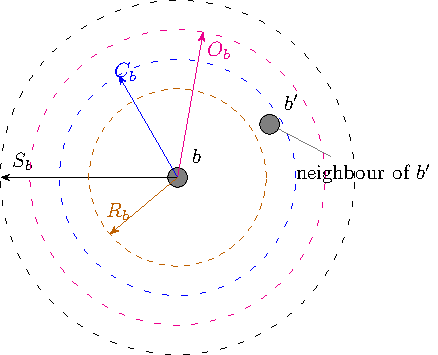
\includegraphics[width=5cm]{figures/stableswarm}
\end{center}
\caption{Agent field ranges. $R_b$ implements repulsion, $C_b$ implements cohesion, $S_b$ is the agent's sensing range, and $O_b$ is used to manage collisions with obstacles. \label{methods:FieldEffects}}
\end{figure}

When cohesion and repulsion are the only field effects used to create a swarming effect, the number of stable structures that can develop is limited {\it (citation needed)}. These structures effectively take the form of either straight edges or partial lattices (Fig.~\ref{concave:SwarmStableShape1}). The maintenance of a well-structured swarm is crucial to their effective deployment in a number of applications, including reconnaissance or artificial pollination, where coverage ``blind spots" are eliminated \cite{elamvazhuthi2015optimal}, and containment, where the swarm is used to surround an object or region \cite{cao2012distributed}.  Over time, the perimeters of partial lattices may contain so-called {\it anomalies}, such as concave ``dents" or convex ``peaks", and these anomalies all contribute to the disruption of an otherwise well-structured swarm. The key, therefore, is to ensure that concave {\it voids} are dynamically removed from a swarm.

\begin{figure}
\begin{center}
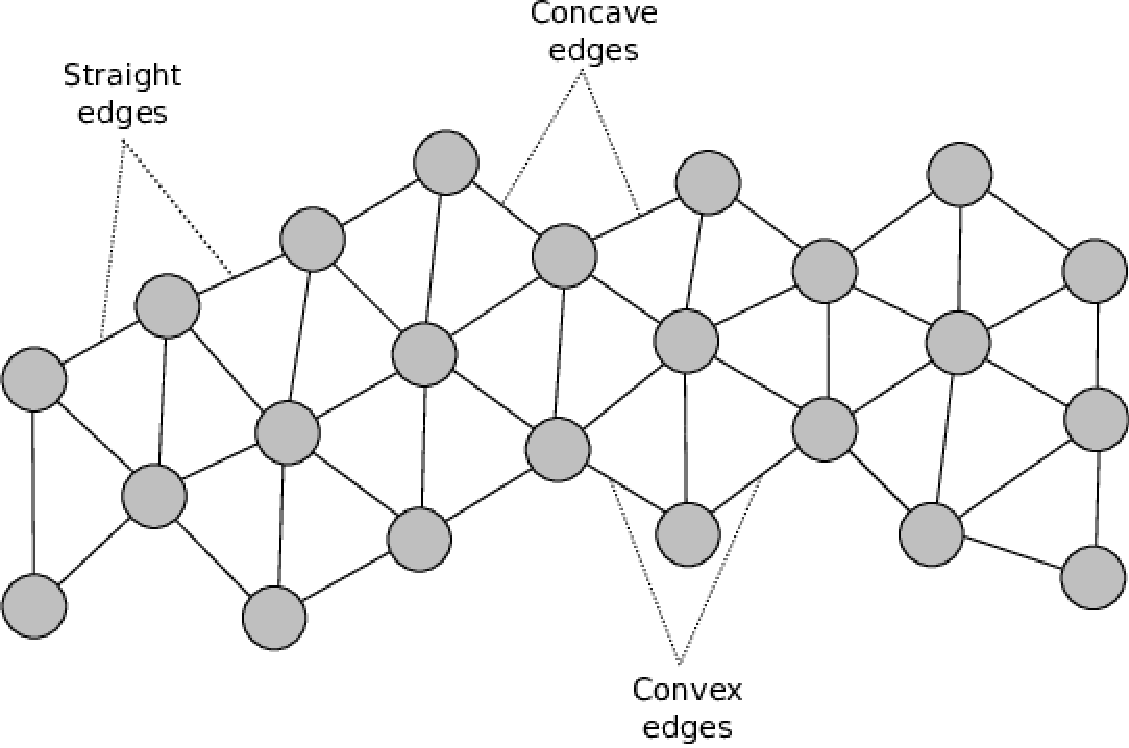
\includegraphics[width=7cm]{figures/SwarmStableShape1}
\end{center}
\caption{Stable swarm structure containing two types of anomaly. \label{concave:SwarmStableShape1}}
\end{figure}

Here, we describe our \textit{void reduction} technique for swarm management, which is a form of self-healing that encourages a swarm to coalesce into a more geometrically stable shape. This is achieved by removing voids and concave edges. Importantly, the techniques defined in this paper function without the need for inter-agent or global {\it messaging} (which can carry a significant overhead), and rely only on local {\it proximity detection}.

The rest of the paper is organized as follows: we first briefly review related work in the area of self-healing swarms, and then describe the baseline swarming model and our novel perimeter detection and void reduction mechanisms.We describe the results of computational studies in a specific application domain (surrounding an oil slick), before we conclude with a brief discussion of our results, and give pointers to possible future work.

\section{Related Work \label{sec:RelatedWork}} 

A prototype framework for self-healing swarms was developed by Dai, {\it et al.}, which considered the problem of agent failure in hostile environments \cite{DHMRZ:06}. This was similar to work carried out by Vassev and Hinchey, who modelled swarm deployment using the ASSL (Autonomic System Specification Language) \cite{VH:09}. This technique was used by NASA (US National Aeronautics and Space Administration) when developing their ANTS (Autonomous Nano Technology Swarm) for use in asteroid belt exploration. However, this work was focused more towards the failure of an agent's internal systems, rather than on the removal of anomalies in a swarm distribution. 

In the context of swarm structure maintenance, Roach, {\it et al.} focussed on the effects of sensor failure, and the impact that has on agent distribution \cite{RMT:15}. Lee and Chong identified the issue of concave edges within swarms in an attempt to create regular lattice formations \cite{GN:08}, and the main focus of their work is the dynamic restructuring of inter-agent formations. Ismail and Timmis demonstrated the use of  \textit{bio-inspired} healing using \textit{granuloma formation}, a biological method for encapsulating an antigen \cite{IT:10}. They have also considered the effect that failed agents can have on a swarm when traversing a terrain \cite{TIBW:16}. 

Our void reduction technique is an extension of the work presented by Ismail and Timmis \cite{IT:10,TIBW:16}, and also builds on the work of Lee and Chong on concave edge identification \cite{GN:08}, and on the work of McLurkin and Demaine on the detection of perimeter types \cite{MD:09}. However, the technique employed in this paper does not explicitly require the identification of the perimeter type, as this would require a communication infrastructure.

\section{Swarm Model}
\label{sec:SwarmModel}

\begin{figure}
\begin{center}
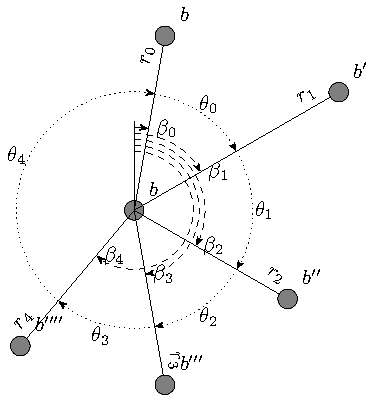
\includegraphics{figures/neighbours}
\end{center}
\caption{Swarm model: representation of interaction with neighbouring agents.  \label{define:neighbours}}
\end{figure}

In this Section, we define the baseline swarm model.  A swarm, $\mathcal S$,  comprises a number of agents; in our application context, each agent is a mobile robot or drone, but this may remain unspecified. An agent $b\in\mathcal S$  has a sensor range, $S_b$,  within which it may detect other agents in the swarm, and determine both their {\it range}, $r$, and {\it bearing}, $\beta$ (Fig. ~\ref{define:neighbours}).  At each time step, the agent generates a set of neighbours, $\mathcal N_b$, comprising other agents that are within a specific range (usually defined as the range of the cohesion field, $C_b$), as given in Equation \ref{set:Nb}. These range and bearing pairs contain the relative position vector for each neighbour, $b'$, with respect to the sensor reference frame of agent $b$. 
This model was defined by Eliot, {\it et. al.} in a paper which introduced a new magnitude-based metric for the analysis of swarms \cite{EKB:18}. 

\begin{equation}
\mathcal N_b = \{ (r,\beta) \ldots \}
\label{set:Nb}
\end{equation}

In order to calculate the new vector, $v$, for $b$, Equation ~\ref{eq:BotPhysics1} defines a weighted model that includes cohesion, repulsion, direction and obstacle avoidance ($v_c(b), v_r(b), v_d(b)$,  and $v_o(b)$, respectively). The weightings $k_c, k_r, k_d, k_o$ allow each component to be scaled in order to tailor the swarming effect. 

\begin{equation}\label{eq:BotPhysics1}
  v(b) = k_cv_c(b) + k_rv_r(b) + k_dv_d(b) + k_ov_o(b)
\end{equation}

\textit{Repulsion}, $v_r(b)$, defined in Equation ~\ref{eq:Repulsion1}, is the directional movement required to prevent agents colliding. $\mathcal R_b$ is defined as the set of agents that are within the repulsion range of $b$.

\begin{equation}\label{eq:Repulsion1}
v_r(b) = 
\frac{1}{\card{\mathcal R_b}}
\left(
	\mathlarger{\mathlarger{\sum_{b' \in \mathcal R_b}}}
	{\left( 1-\frac{\magn{b'}}{R_b} \right)}
	b'
\right)
\end{equation}

\textit{Cohesion}, $v_{c}(b)$, defined in Equation ~\ref{eq:FlyToCentre1}, calculates the movement required to make an agent move towards other agents in order to form a cohesive structure. $\mathcal C_b$ is defined as the set of agents that are within the cohesion range of $b$.

\begin{equation}\label{eq:FlyToCentre1}
	v_c(b) =
	\frac{-1}{\card{\mathcal C_b}}\left({\mathlarger{\sum_{b' \in
	\mathcal C_b}}{b'}}\right)
\end{equation}

\textit{Direction}, $v_d(b)$, defined in Equation ~\ref{eq:Direction}, generates a directional vector for an agent to move towards some destination, $d$.

\begin{equation}
\label{eq:Direction}
v_d(b) = d
\end{equation}

{\it Obstacles}, like agents, may be represented as a point. As an agent moves, it may enter an obstacle's \textit{repulsion field}. If this occurs, then the agent should move away (as we assume that an obstacle is unable to take evasive action itself). Here, agents have a fixed \textit{obstacle repulsion field}, $O_b$. If an obstacle enters the field, a vector of magnitude $O_b$ is applied. If more than one obstacle is present within the field, the applied repulsion vector is the sum of the repulsion vectors (Figure ~\ref{fig:Obstacle1}). The resultant vector is normalised and scaled such that the magnitude is the same as the field distance, $O_b$, as given in Equation ~\ref{eq:Obstacle2}.

\begin{figure}
\begin{center}
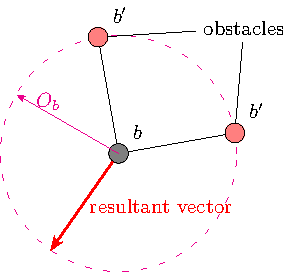
\includegraphics{figures/obstacles}
\end{center}
\caption{Repulsion from obstacles. \label{fig:Obstacle1}}
\end{figure}

Equation ~\ref{eq:Obstacle2} shows the repulsion vector, $v_o(b)$, for an agent. $\mathcal O_b$ is the set of obstacles within the range of agent $b$. The obstacles are identified by comparing their Cartesian distance to the fixed obstacle repulsion field $O_b$, so $\forall o \in \mathcal O_b : \magn{o}\leq O_b$. The applied repulsion is calculated by scaling the normalised sum of the normalised vectors $\hat o$ by $O_b$.  Note that $\string^$ is the equivalent of $\hat v = \frac{v}{\magn{v}}$, the normalised vector.

\begin{eqnarray}\label{eq:Obstacle2}
  v_o(b) & = & O_b \hat q_o \\
	\mathrm{where~}  q_o & = & \sum_{o\in \mathcal O_b } \hat o
	\nonumber \\
	v_o(b) & = & O_b \left(\sum_{o\in \mathcal O_b }\hat o\right)^{\!\!\wedge} \nonumber
\end{eqnarray}

An agent's \textit{movement vector} is defined as the sum of all the component vectors, as shown in Equation~\ref{eq:BotPhysics1} (similar to that used by Hashimoto, {\it et. al.} \cite{HAY:08}). In order for a vector to be used for movement, it must be normalised before the agent's speed, $s_b$, can be applied. The resulting movement vector, $m_b$, is defined in Equation~\ref{eq:AgentMovement}, and is calculated using unit time, speed and the normalised \textit{movement vector}.

\begin{equation}\label{eq:AgentMovement}
m_b = s_b  \hat v(b)  t
\end{equation}

Over time, applying the calculations described in this Section to all agents in turn creates the global swarming effect. This provides the {\it baseline} algorithm for swarm movement.
We now describe how the swarm may be {\it dynamically reconfigured}, which is the main novel contribution of this paper. After describing our new algorithm for void reduction, we show how it may be applied to a specific problem.
  
\subsection{Perimeter Detection}
\label{sec:PerimeterDetection}

In order to dynamically restructure a disorganised swarm, we must first identify the {\it perimeter} agents. This is due to the fact that anomalies occur at at swarm boundary locations. With reference to Fig.~\ref{fig:PerimeterBots1}, these agents may form part of an outer ({\color{green}green}) or inner ({\color{red}red}) edge.

Our detection mechanism detects both the outer edge of a swarm (Equation \ref{perimeter-predicate}) and any internal features (voids) that satisfy the same set of conditions. It is therefore possible to have both voids and ``islands" of agents within the same swarm. Voids are best defined as perimeters that are both concave (Equation \ref{concave-predicate}) in nature and which exist inside another perimeter. McLurkin \cite{MD:09} describes two types of perimeters, convex and concave, where a convex perimeter is an edge where the average angle of the exposed faces of relevant agents is ~$> 180^\circ$, and a concave perimeter is one where the average exposed angle is~$< 180^\circ$.

\begin{figure}
\begin{center}
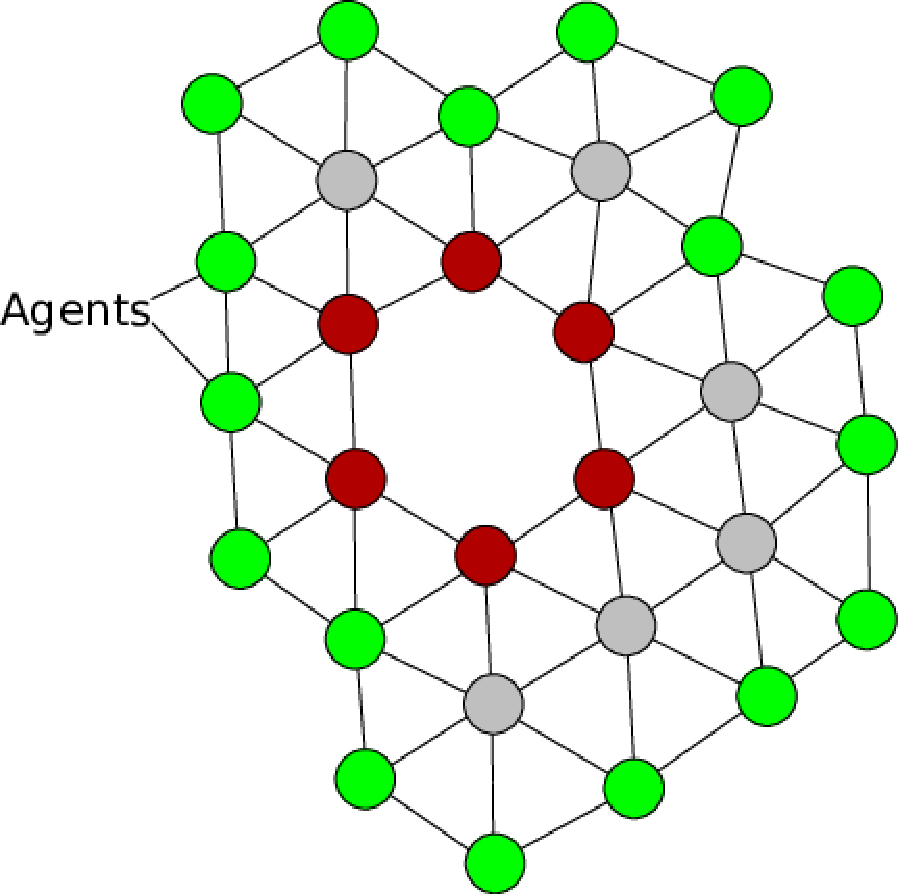
\includegraphics[width=5cm]{figures/PerimeterBots1}
\end{center}
\caption{{\color{green}Outer} and {\color{red}inner} swarm perimeters. \label{fig:PerimeterBots1}}
\end{figure}

% \begin{figure}
% \begin{center}
% \includegraphics[width=4cm]{figures/PerimeterBots2}
% \end{center}
% \caption{Inner Island Perimeter\label{fig:PerimeterBots2}}
% \end{figure}


The set of neighbours, $\mathcal N_b$ (Equation \ref{set:Nb}) is sorted into the sequence $\mathcal P_a$, in ascending order of bearing: 

\begin{equation}
	\mathcal P_a = \langle (r_0,\beta_0),\ldots,(r_n,\beta_n) \rangle
\end{equation}
such that $\beta_0 < \beta_1 < \ldots < \beta_n$

This set of agents forms the perimeter of an enclosing polygon of agent $b$. Each consecutive pair of agents in the sequence defines an {\it edge}, which has length $d$ and an angle $\theta$ given by the difference in bearings of successive neighbours. The sequence of edges that forms this polygon is:

\begin{equation}
	\mathcal{P}_e = \langle (d_0,\theta_0), \ldots , (d_n,\theta_n) \rangle
\end{equation}
where
\begin{equation}
	\theta_i = \beta_{i+1} - \beta_i
\end{equation}

The index addition is modulo $|\mathcal N_b|$, making $\beta_0$ the successor bearing to $\beta_n$ ($n+1 = 0$).  The angles $\theta$ must lie in the range $0<\theta\leq2\pi$. This restriction on the values of $\theta$ enforce the condition that

\begin{equation}
	\sum\theta_i = 2\pi
\end{equation}

The length of a perimeter edge is given by the cosine rule

\begin{equation}
	d_i^2 = r_{i+1}^2 + r_i^2 -2r_{i+1}r_i \cos\theta_i
\end{equation}

An agent is therefore on the perimeter of the swarm if it is not enclosed by the polygon defined in $\mathcal{P}_e$.  Simple geometry shows that this is the case, given by the predicate in Equation ~\ref{enclosing}.

\begin{equation}
	\exists \theta_i \in \mathcal{P}_e : \theta_i\geq\pi
	\label{enclosing}
\end{equation}

The polygon is considered to be ``open" if two successive agents on the perimeter are unable to ``see" one another; that is, their separation, $d$, is greater than the range of the attractive field.  An open polygon does not enclose the agent $b$, so it is considered to be on the perimeter. 

Formally, a agent, $b$, is on the perimeter of the swarm if the predicate in Equation ~\ref{perimeter-predicate} is true.

\begin{equation}
	\exists d_i\in\mathcal{P}_e:d_i>C_b \vee
	\exists\theta_i\in\mathcal{P}_e:\theta_i\geq\pi
	\label{perimeter-predicate}
\end{equation}

An agent is at the apex of a concave region of the perimeter if

\begin{equation}
	\exists(\theta_i,d_i)\in\mathcal{P}_e : d_i>C_b\wedge\theta_i<\pi
	\label{concave-predicate}
\end{equation}

The orientation is independent in so much as: if the agent $b$ is rotated through an angle of $\gamma$ then the bearings are rotated by $-\gamma$, \[ \beta_i\mapsto\beta_i-\gamma \] The  angle between successive agents is now
\[
	\theta_i  =  (\beta_{i+1}-\gamma) - (\beta_i-\gamma)
	 = \beta_{i+1}-\beta_i-\gamma+\gamma
	 = \beta_{i+1}-\beta_i
\]

\subsection{Void Reduction}

In a static swarm, where there are essentially no \textit{destination vectors}, void reduction will result in a restructuring motion that creates a more  ``rounded' swarm. Void reduction also creates a {\it surrounding} effect, as it removes voids from a swarm. This is discussed in more detail in the next Section.  Although these effects improve the potential applications of swarms, negative effects may also be introduced (e.g., in some circumstances void reduction can create an artificial \textit{destination vector}, in that the swarm will appear to have a directional movement). 

In order to implement void reduction, full perimeter detection is required in order to identify candidate agents. Void reduction does not require the perimeter {\it type} to be identified,  and no communications infrastructure is required. Many existing swarm coordination algorithms require the availability of inter-agent communication \cite{JG:13,MD:09,SOM:12,NIM:09,ZFG:13}, and this imposes a significant limitation on swarm size due to the requirement for message propagation. Our method avoids the problems associated with this.

\subsection{Void Reduction: Agent Movement}\label{concave:AgentMovement}

Adding a further characteristic to the motion of a swarm necessitates a revision to the existing agent model ~(Equation ~\ref{eq:BotPhysics1}). With void reduction, this revision is based on the identification of the agents that are connected by a concave edge, as shown in Fig.~\ref{concave:VoidConcave1} as $(b^{'},b,b^{''})$. 

\begin{figure}
\begin{center}
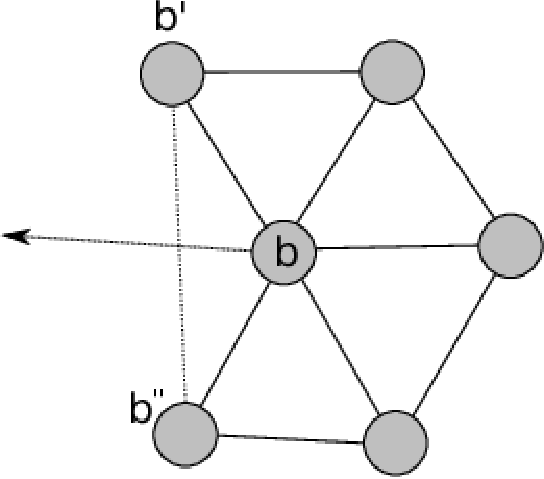
\includegraphics[width=4cm]{figures/VoidConcave1}
\end{center}
\caption{Agent void reduction motion: agents $b'$ and $b''$ form a concave edge (depicted by the lighter line). Agent $b$ must therefore move to remove this edge. \label{concave:VoidConcave1}}
\end{figure}

When an agent is identified as being a component of a concave characteristic (Equation ~\ref{concave-predicate}) the normal \textit{movement-direction vector} is replaced by a \textit{void reduction vector}. This new vector causes the agent to move in a direction that will reduce or remove a concave edge by moving the agent towards the identified gap. The effect of this will be to either straighten an outer perimeter or reduce/remove a void. This change in direction affects the distance and magnitude variances due to the changes induced. Figure ~\ref{fig:InterAgentEffect}  shows this effect in more detail; the top figure shows the initial positions of the agents before void reduction is applied to the agent, and the bottom part of the figure shows the effects on its relationship with its neighbours. The aggregate change is an increase in the inter-agent distances, and an increase in the resultant magnitude effects.

\begin{figure}
\begin{center}
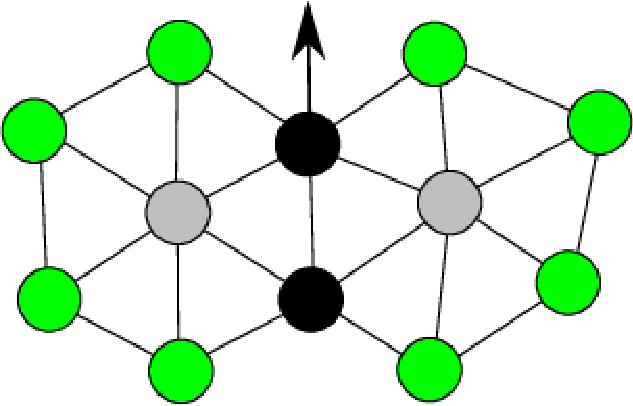
\includegraphics[width=5cm]{figures/InterAgentEffect1}
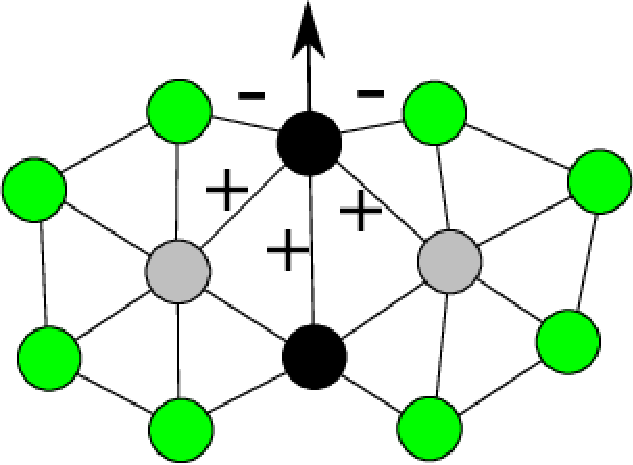
\includegraphics[width=5cm]{figures/InterAgentEffect2}
\end{center}
\caption{Initial position (top), and reduced position (bottom). +/- labels show relative changes in inter-agent magnitude. \label{fig:InterAgentEffect}}
\end{figure}


\section{Experimental Results: Oilslick Containment}
\label{voids:ObjectSurrounding}

In this Section we give the results of experiments to simulate a specific scenario; that of {\it oilslick containment} using a mobile robot swarm. Oil spills (from ships or drilling operations) can cause significant environmental, social and economic damage, and removing them can be hazardous and expensive. Several alternatives to traditional spill dispersal/containment procedures have been proposed, with some proposals relying on the use of robot swarms to surround a spill \cite{fritsch2007control,kakalis2008robotic,ZFG:13} (details of remediation processes are outside the scope of this paper, but they may include skimming of the surface, deposition of a dispersal agent, or oil containment using a boom). However, these proposals all require the use of a communications infrastructure to facilitate message passing between agents. Our proposed method has the {\it significant benefit} of not requiring any such mechanism, relying only on local proximity detection.


 \begin{figure}
 \begin{center}
 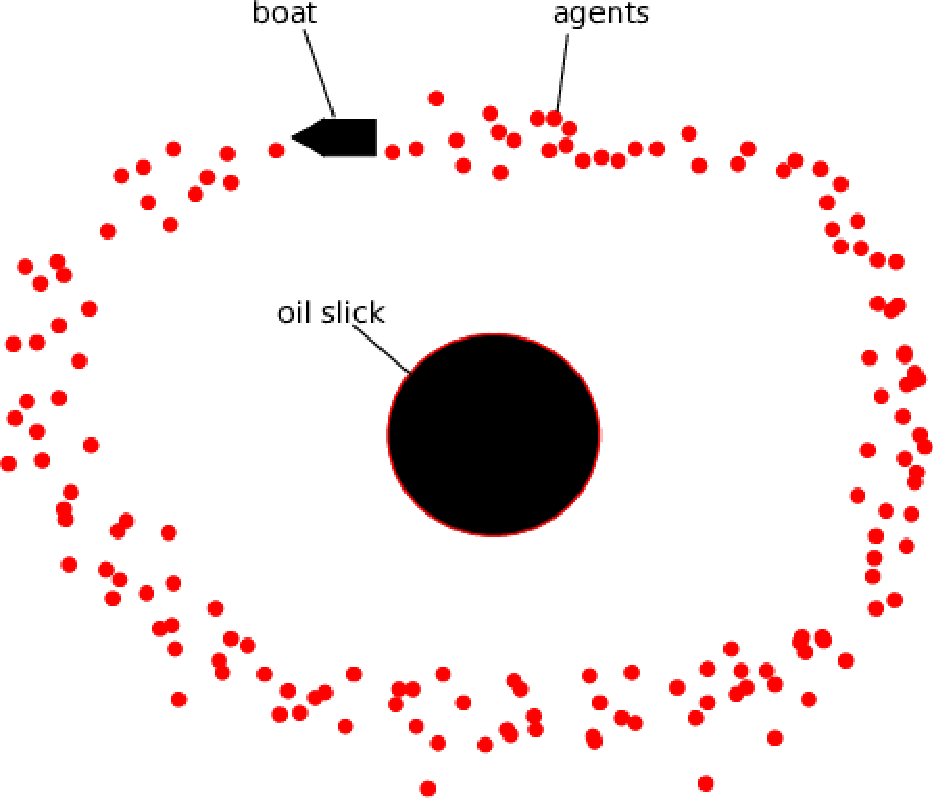
\includegraphics[width=6cm]{figures/OilSlick}
 \end{center}
 \caption{Oil slick containment scenario. \label{voids:OilSlick}}
 \end{figure}

%Figure~\ref{concave:OilSpillSimulation} is a screen shot of the deployment within the simulator for testing this hypothesis. 
%
% \begin{figure}
% \begin{center}
% \includegraphics[width=8cm]{figures/OilSpillSimulator}
% \end{center}
% \caption{Oil spill containment simulation\label{concave:OilSpillSimulation}}
% \end{figure}

The scenario is schematically depicted in Fig.~\ref{voids:OilSlick}; we have an oil slick in some environment, and a swarm of robots that are deployed by boat around the perimeter of the slick.
Figure~\ref{spillresults} shows the results of simulating the containment process using both the baseline movement algorithm (top) and the baseline method with void reduction (bottom). In our simulation, we use 200 agents, which is significantly greater than the number of agents than are generally simulated when inter-agent communication is required.

Without void reduction (i.e., simply using the field-effect-based movement algorithm) the swarm expands and then stabilises into a structure containing a void.  The swarm ``vibrates" slightly as cohesion and repulsion forces fluctuate to maintain the swarm's structure, but the void does not fully close, and full close containment is not achieved. The agents that do come in contact with the obstacle are repelled by the obstacle repulsion field. If, however, we activate void reduction, then the swarm expands as expected, due to the field effects, but then the void is completely removed, achieving full and close containment of the slick.

\begin{figure*}
  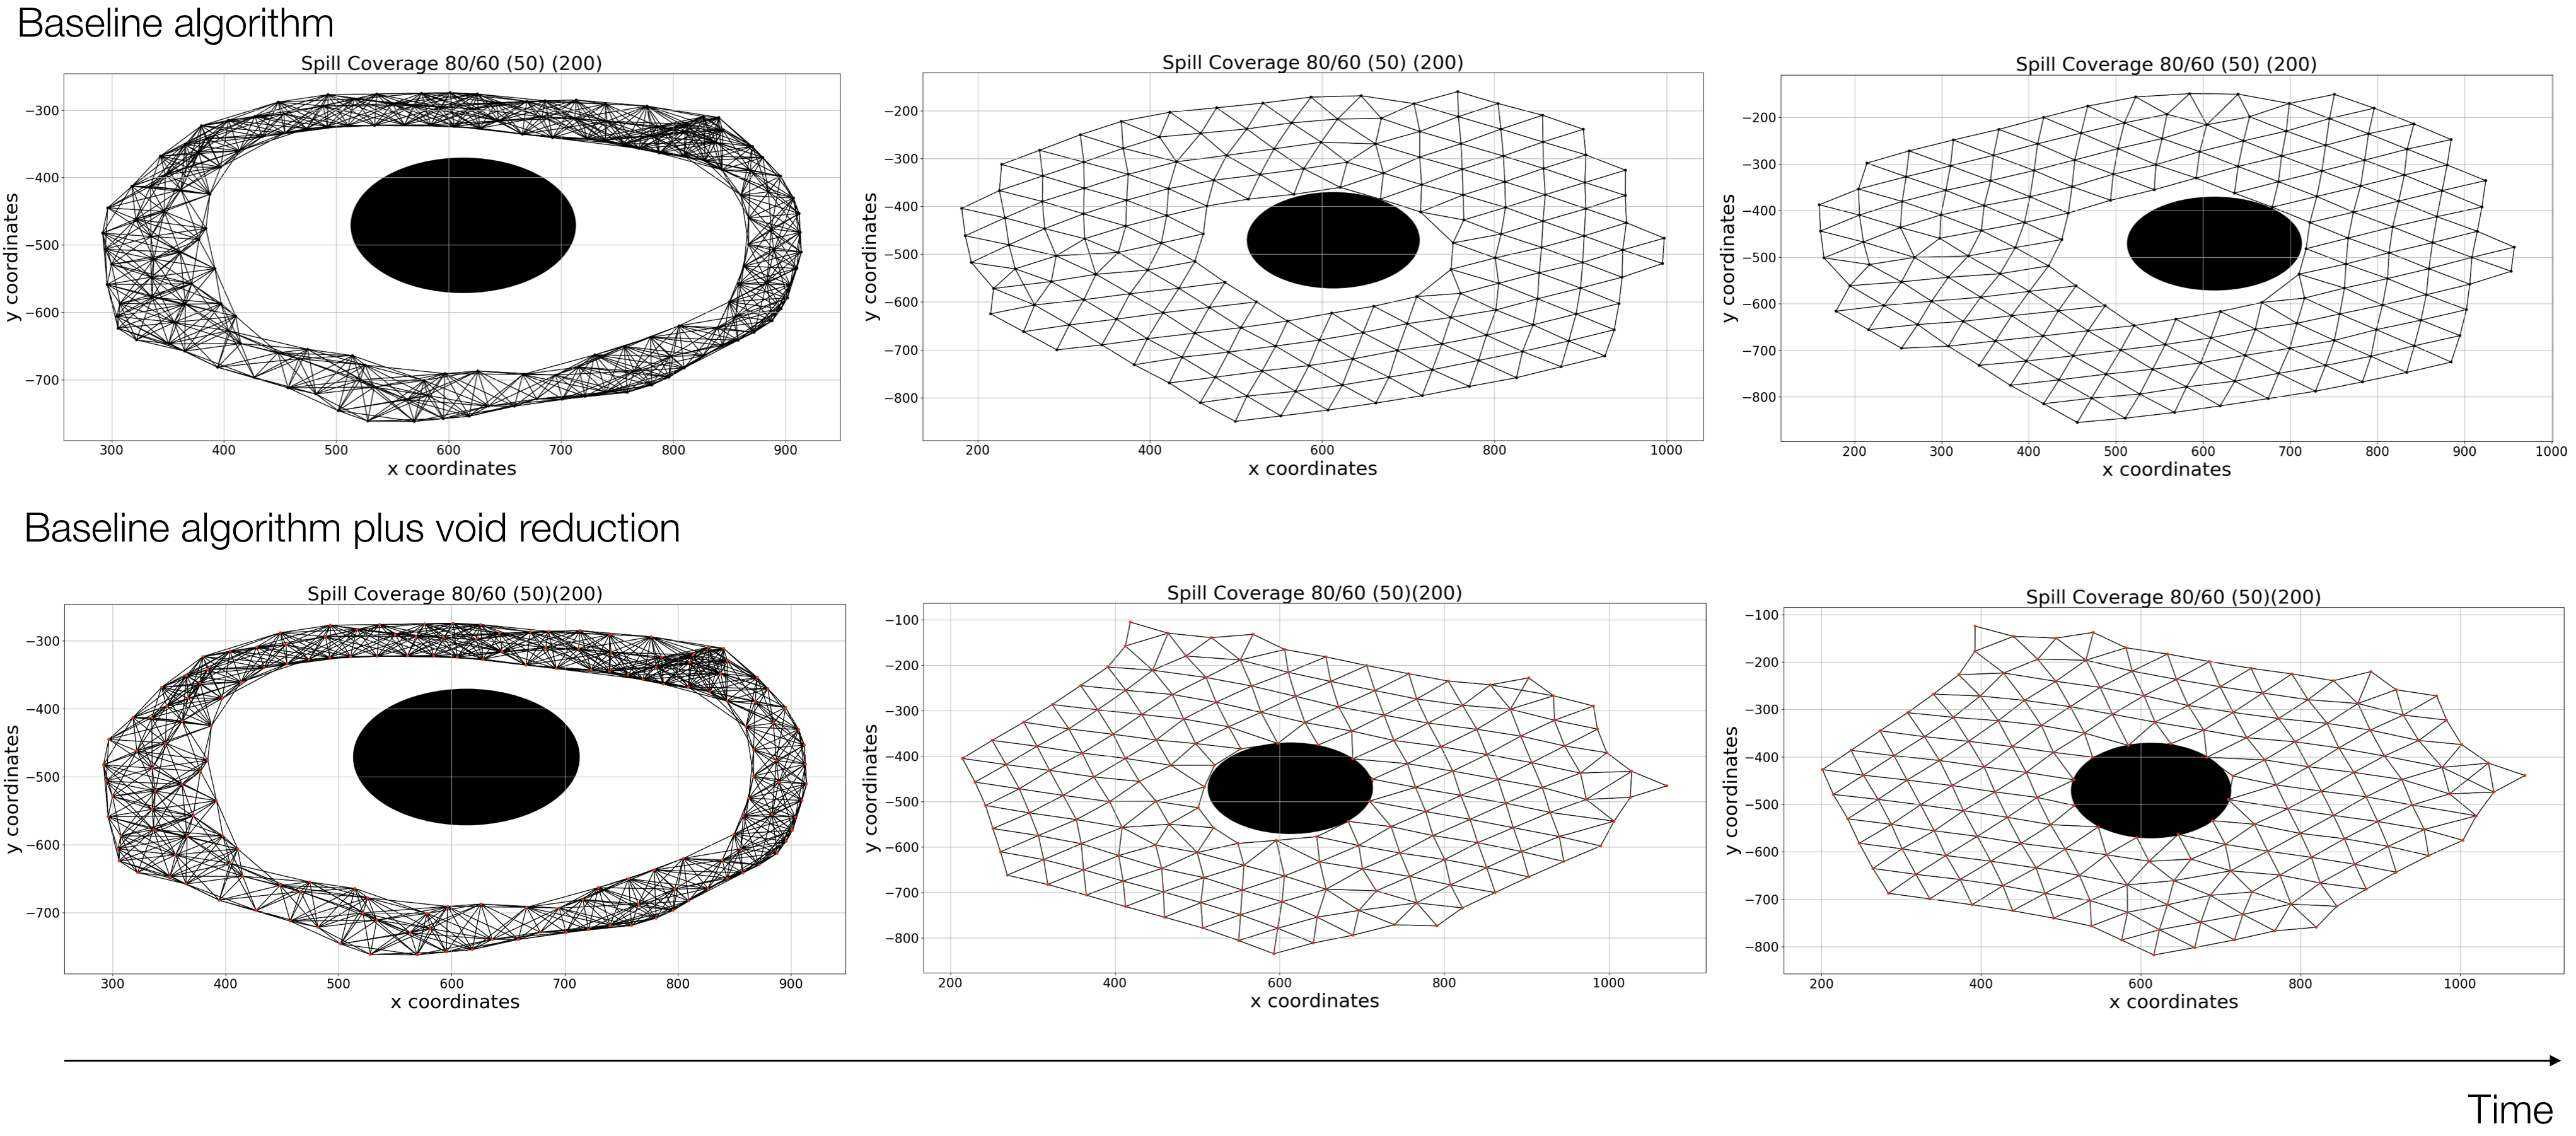
\includegraphics[width=\textwidth]{figures/spillresults}
  \caption{Simulation results for oil slick containment scenario. Top three frames show the evolution of the swarm using only the baseline movement algorithm; bottom three frames show the impact of adding our void reduction method.}
  \label{spillresults}
\end{figure*}


Figures ~\ref{concave:OilSpillPerimeter8060-DIST-1} and \ref{concave:OilSpillPerimeter8060-MAG-1} show the effect of the void reduction on the distribution of agents compared to the baseline method. Figure~\ref{concave:OilSpillPerimeter8060-DIST-1} shows the distance distribution of the swarm for both the baseline method (grey/black) and the void reduction method (red). The baseline swarm initially expands, then settles after approximately 6 seconds (this is also the case for the void reduced swarm). Following the initial expansion, the baseline swarm remains relatively slow-changing with respect to distance and magnitude. However, the void reduced swarm is affected more significantly; after approximately 10 seconds the swarm's internal void perimeter makes contact with the oil spillage (obstacle). This has the effect of disrupting the average distance and average \textit{inter-agent magnitudes}. This effect diminishes slightly after approximately 18 seconds, when the swarm's \textit{void reduction vectors} cause the swarm to surround the spillage. The slick surrounding process is followed by a few remaining changes caused by the ``snapping" of agents at the spillage perimeter, and then the containment process is complete.

 \begin{figure}
 \begin{center}
 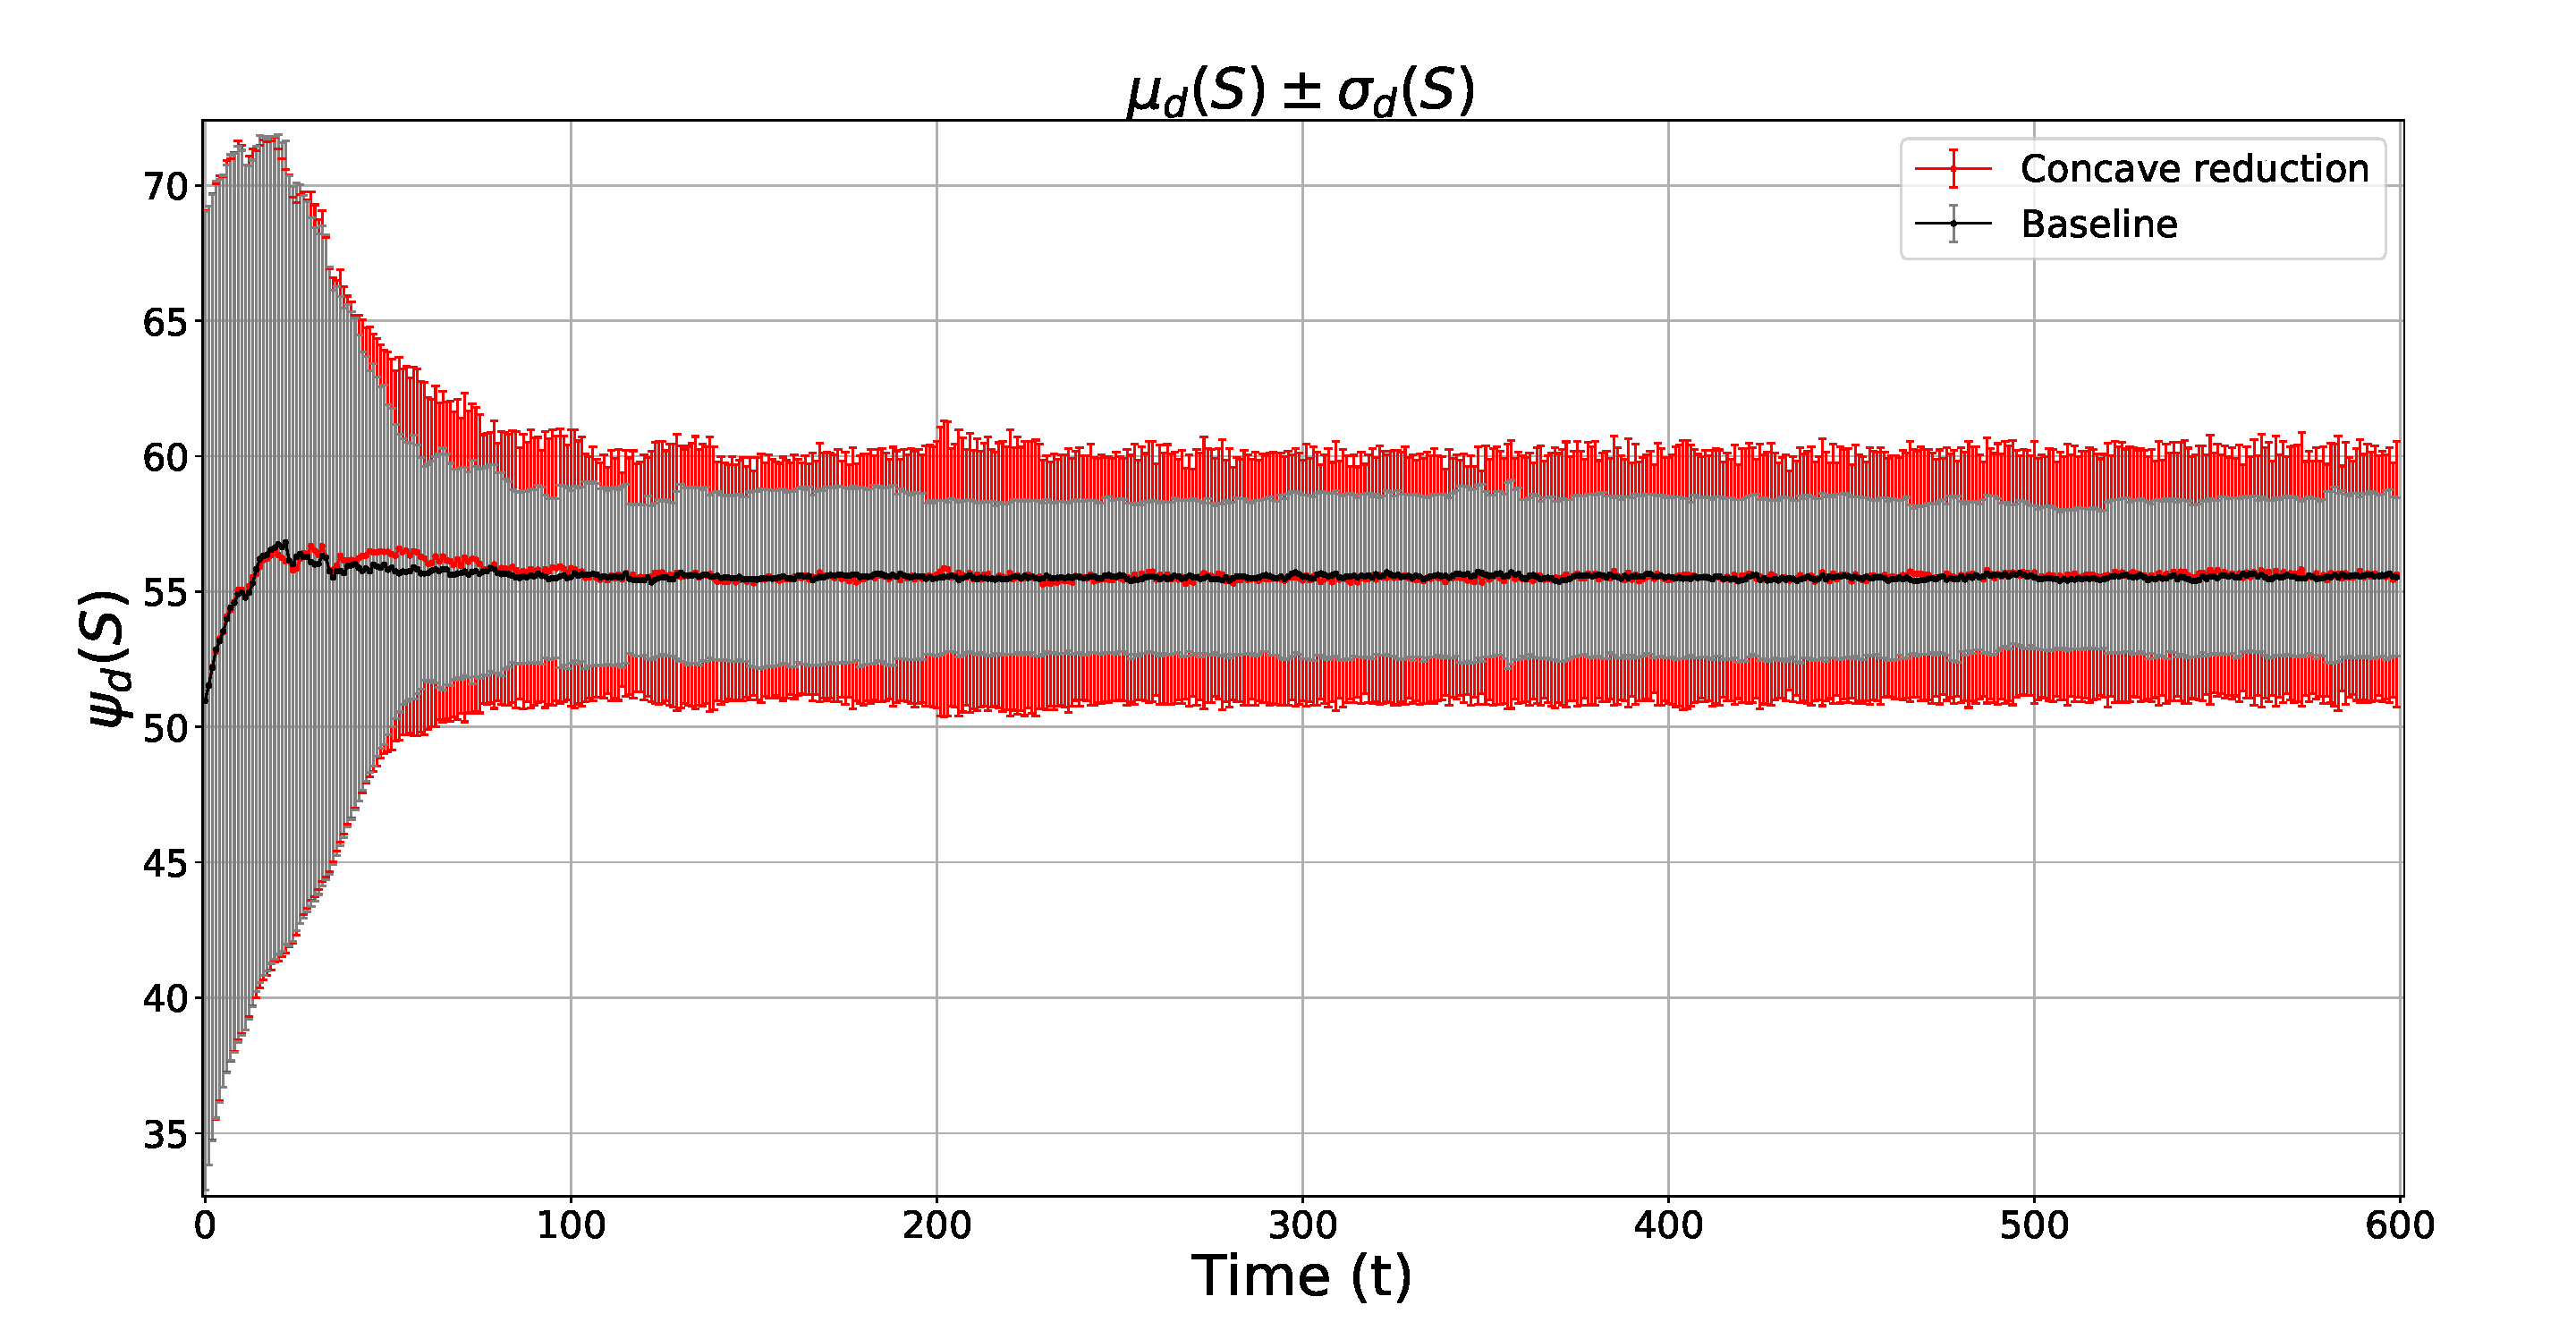
\includegraphics[width=8cm]{figures/OilSpillPerimeter8060-DIST-1}
 \end{center}
 \caption{Oil spill containment distance (time shown in milliseconds (ms)). \label{concave:OilSpillPerimeter8060-DIST-1}}
 \end{figure}

Figure~\ref{concave:OilSpillPerimeter8060-MAG-1} compares \textit{inter-agent magnitudes} for the baseline and void reduction swarms. When initially deployed, the swarm is so dense that the average \textit{inter-agent magnitude} is negative, indicating a high level of expansion. Within 2 seconds the expansion has reached a point where the average magnitude is positive, indicating the swarm is cohesive. This means that the swarm will remain as a single entity, and therefore be capable of surrounding an object without breaking apart.

 \begin{figure}
 \begin{center}
 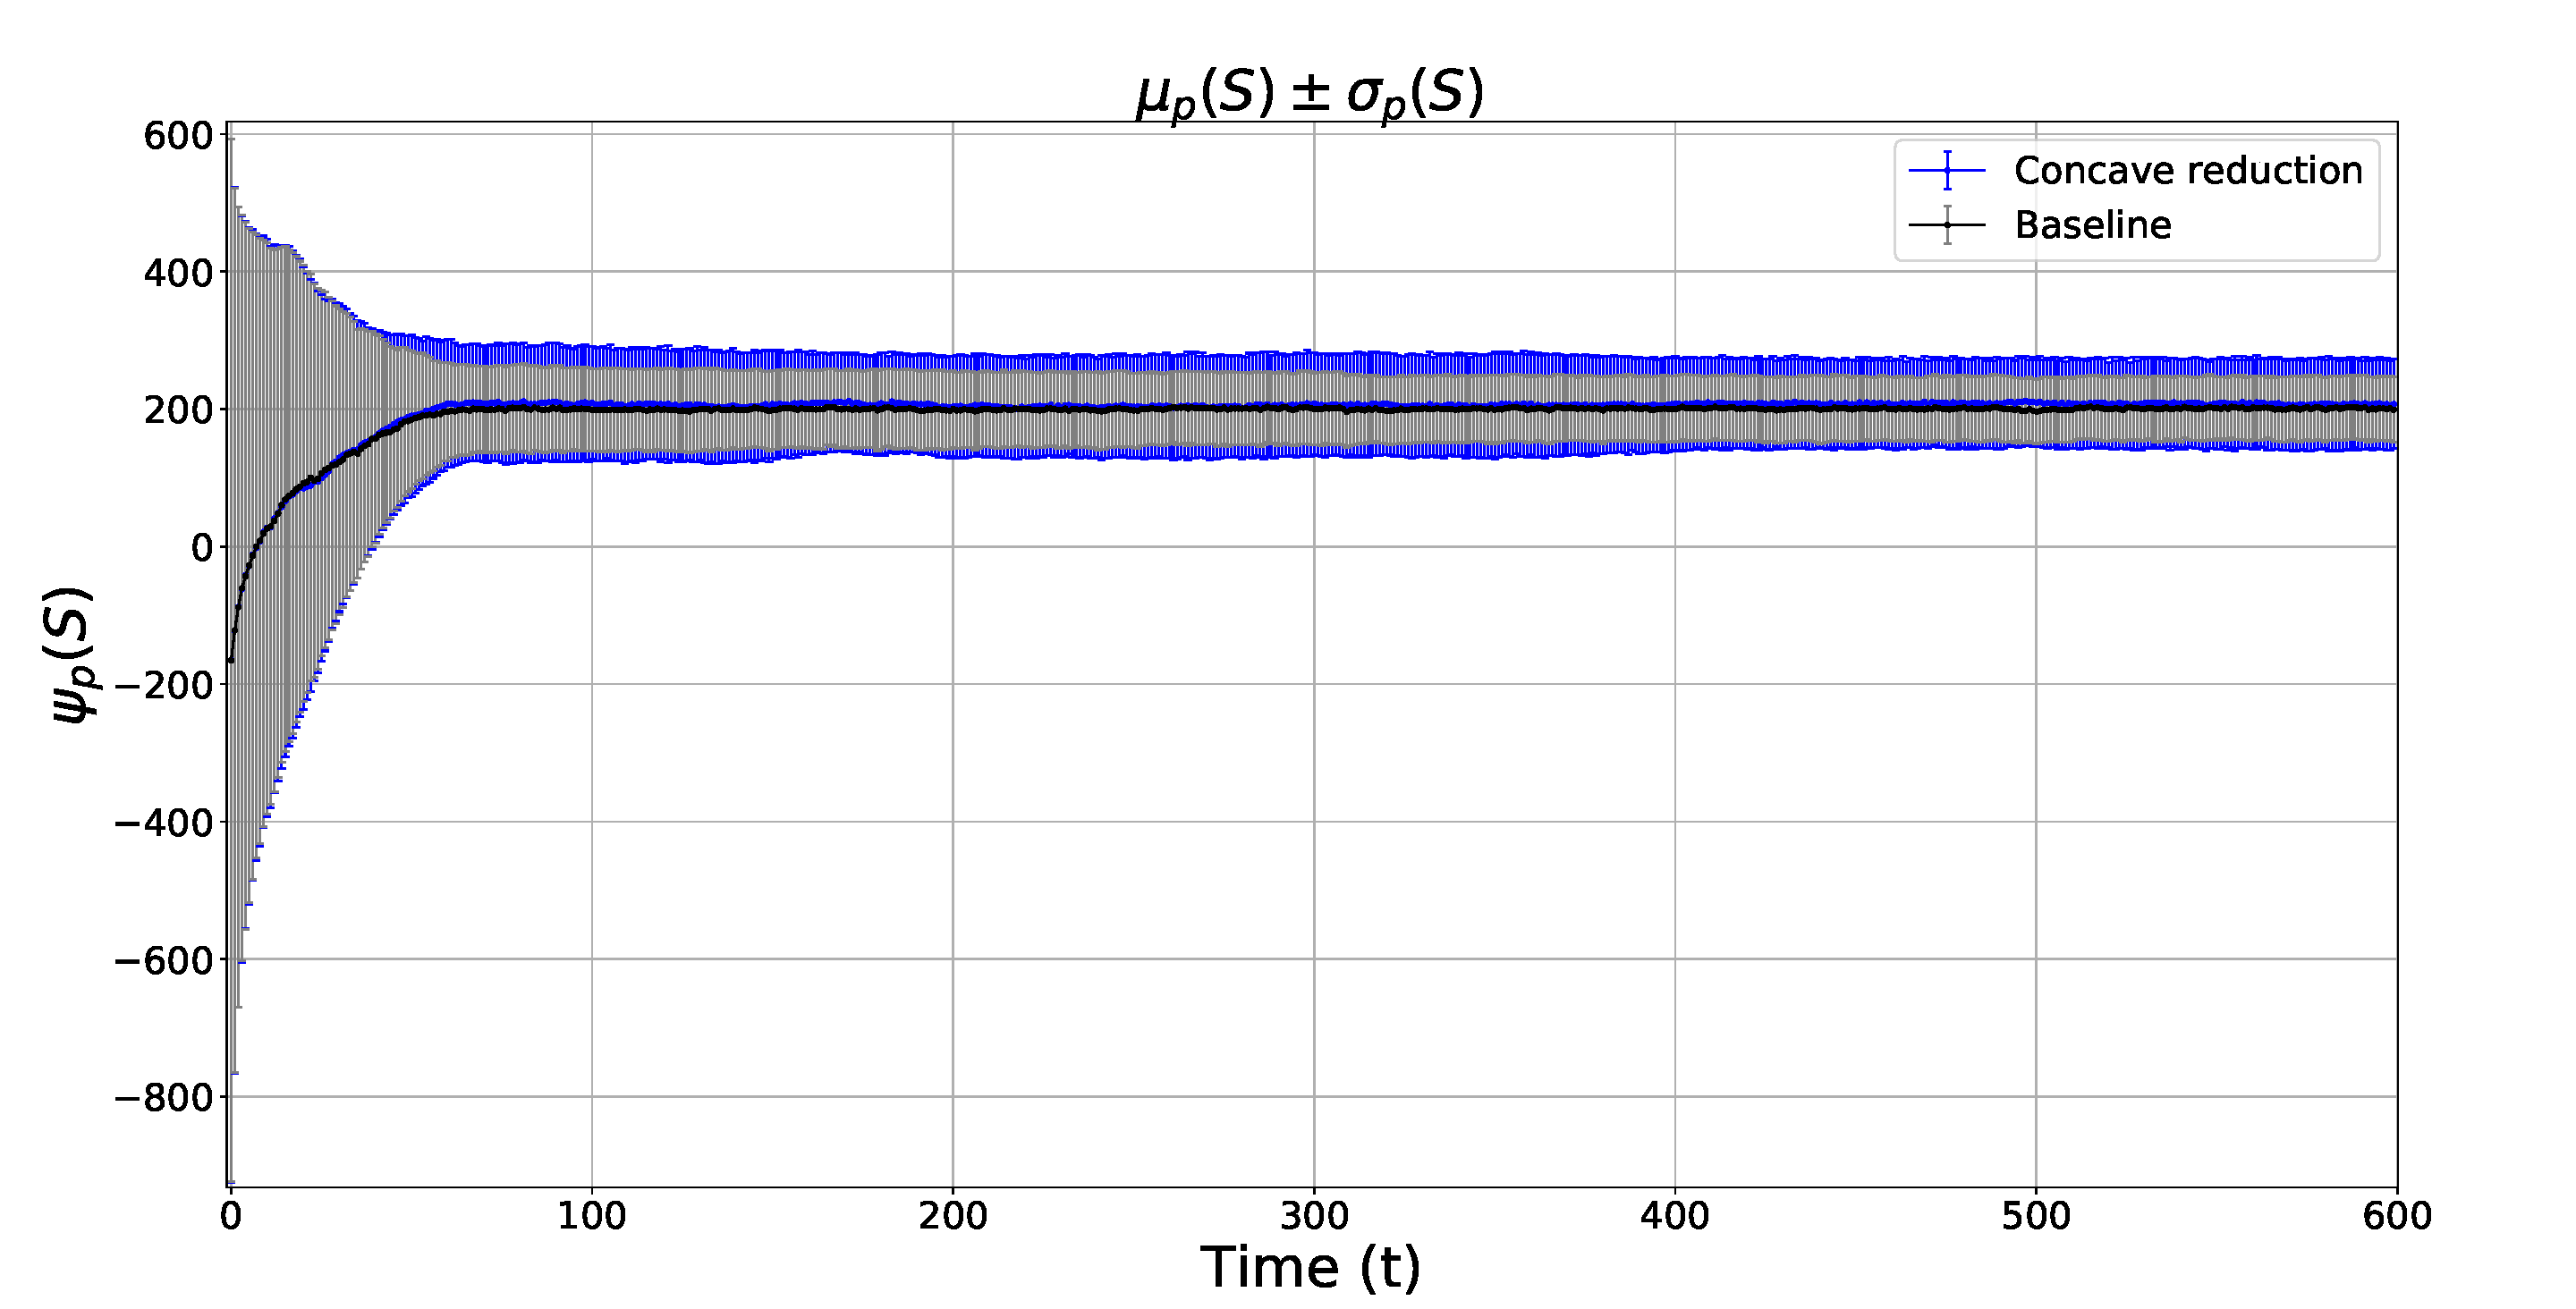
\includegraphics[width=8cm]{figures/OilSpillPerimeter8060-MAG-1}
 \end{center}
 \caption{Oil spill containment magnitude (time shown in milliseconds (ms)). \label{concave:OilSpillPerimeter8060-MAG-1}}
 \end{figure}

When the swarm shrinks to surround the obstacle, we see an erratic change in the number of perimeter agents. Figure~\ref{concave:OilSpillPerimeter8060-1} shows the number of perimeter agents over the duration of the simulation. We see that the baseline swarm perimeter size decreases steadily and then settles (the swarm has not enclosed the spillage). The perimeter count has settled, but, as shown in Fig.~\ref{concave:OilSpillPerimeter8060-DIST-1} and \ref{concave:OilSpillPerimeter8060-MAG-1}, the agents are still moving (magnitude variance and magnitude \textgreater 0); however, the movement does not affect the overall structure. 

When the void reduction swarm encounters the obstacle at approximately 100 ms there is a change due to ``snapping", as the agents ``fold" around the obstacle. Snapping is an oscillation of relations between four agents. The perimeter size then continues to fall gradually as the void percolates out of the system. The perimeter size then stabilises as the slick obstacle is fully surrounded.

 \begin{figure}
 \begin{center}
 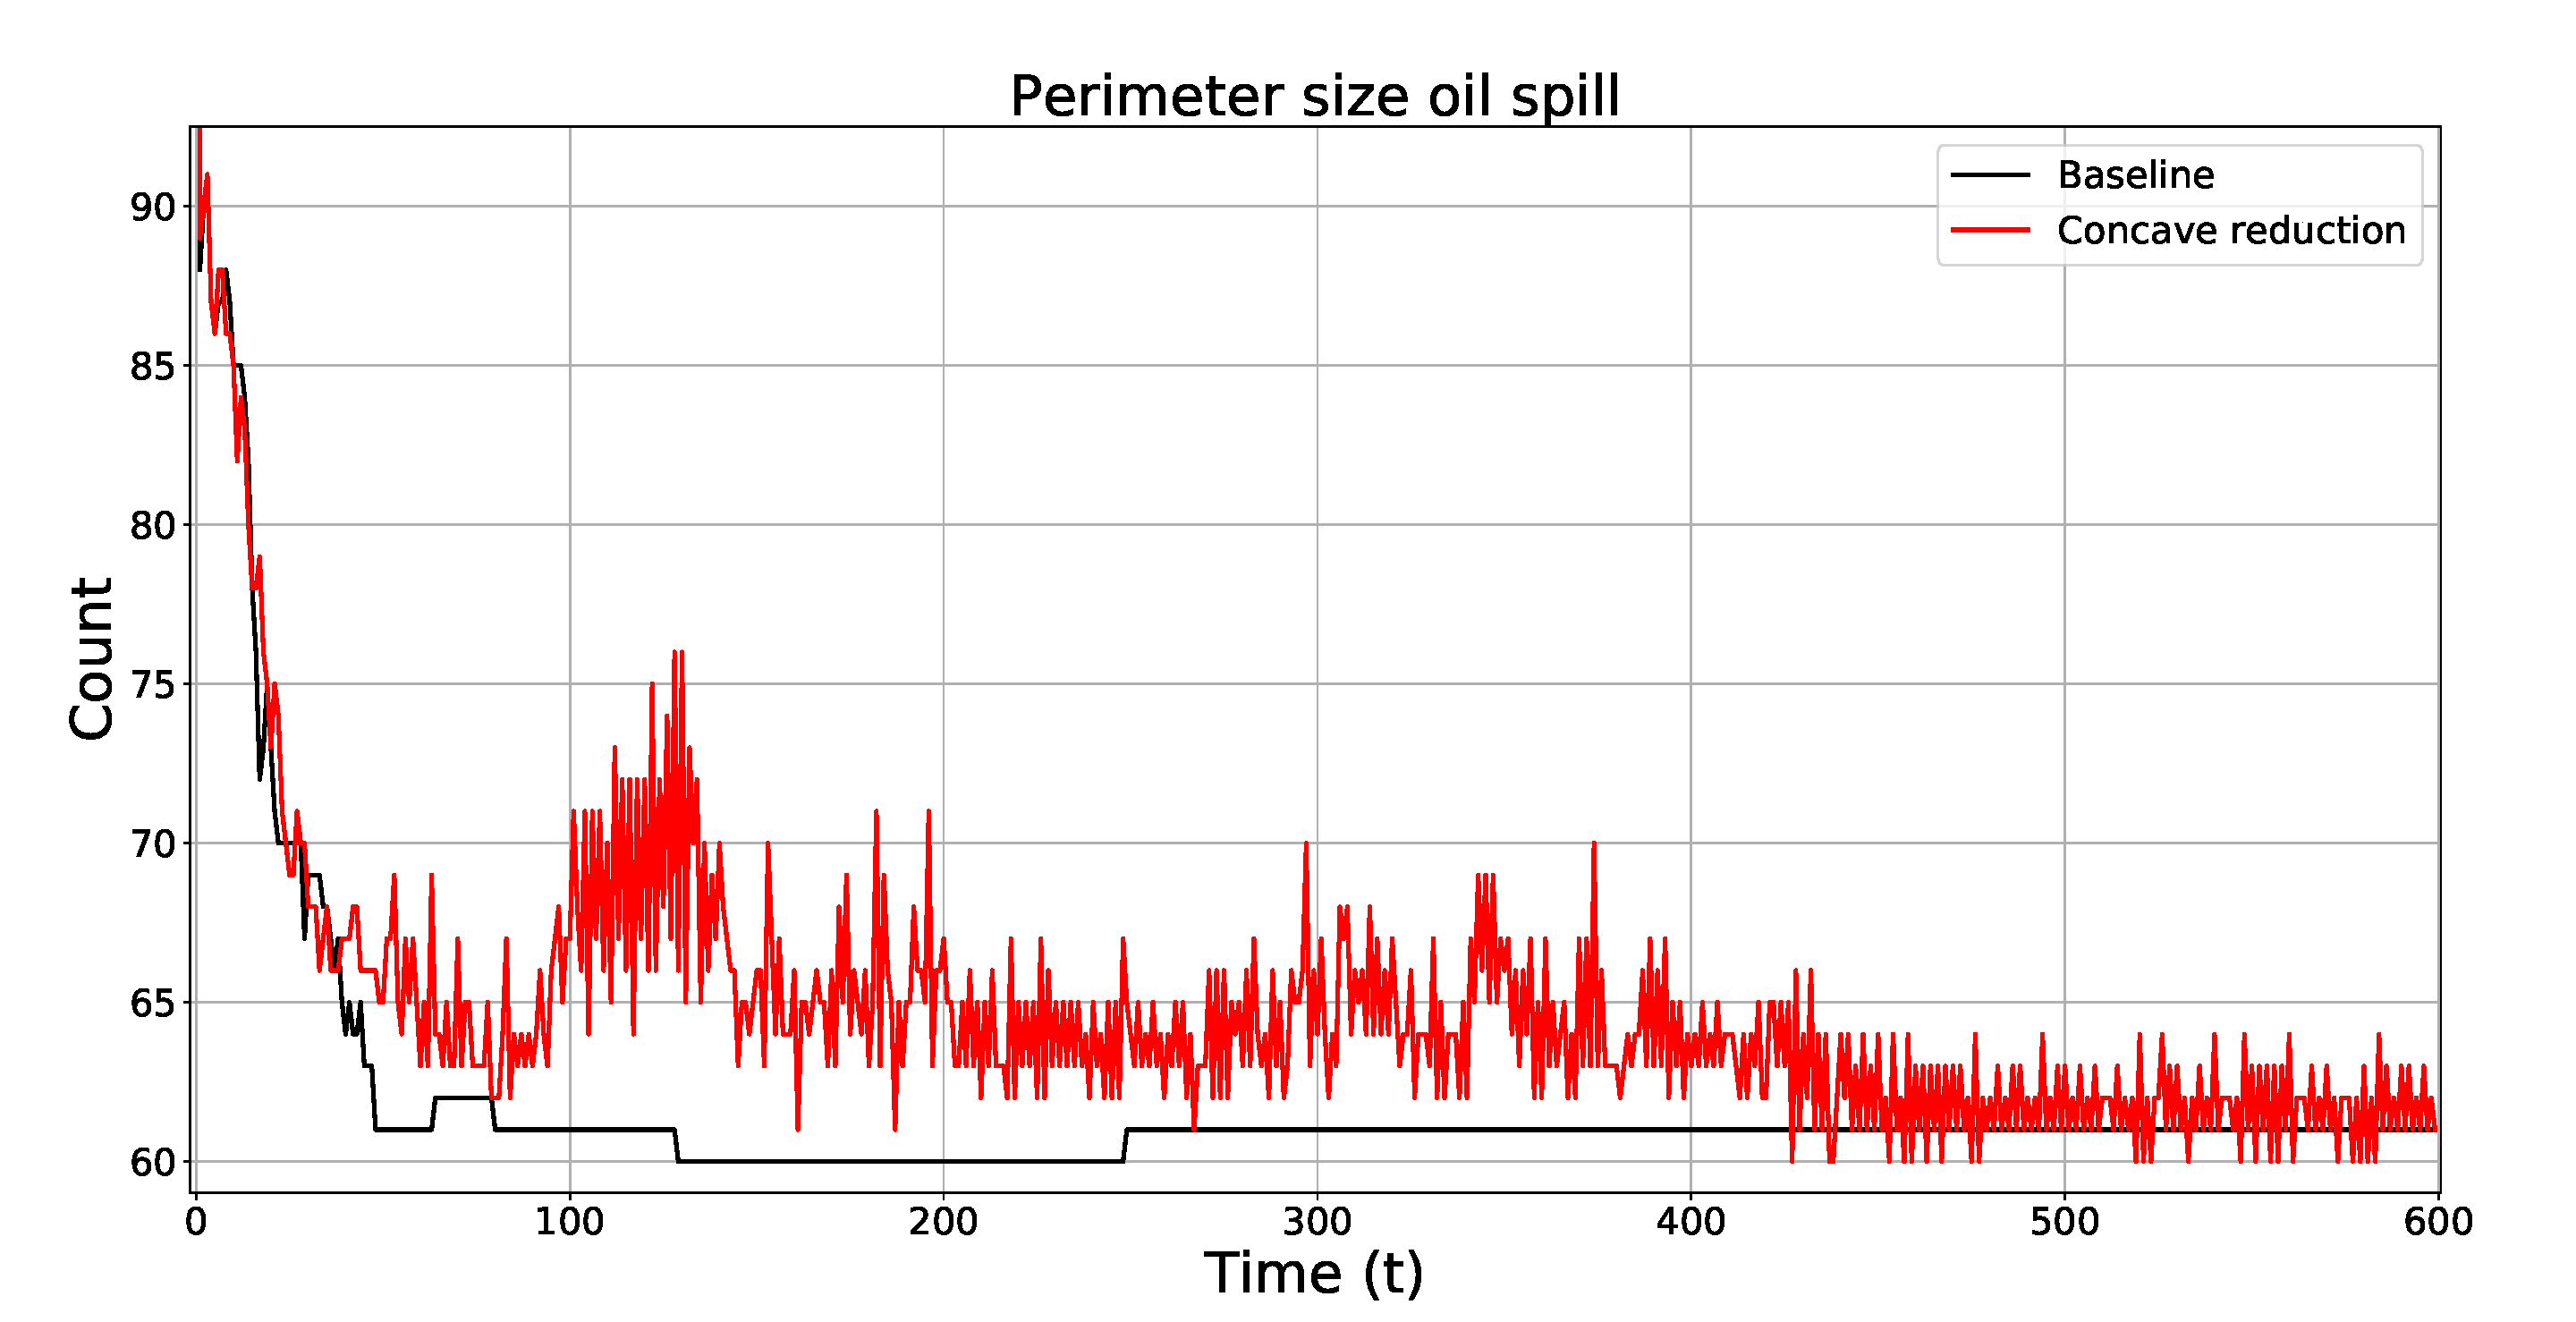
\includegraphics[width=8cm]{figures/OilSpillPerimeter8060-1}
 \end{center}
 \caption{Swarm perimeter size comparison (time shown in milliseconds (ms)). \label{concave:OilSpillPerimeter8060-1}}
 \end{figure}

\section{Conclusion}
\label{voids:Conclusion}

In this paper, we have shown how the structure of a simulated swarm of robots may be controlled by the identification and removal of perimeter anomalies. Importantly, the identification of anomalies is achieved locally by individual agents using only proximity detection, without any need for an inter-agent communication structure. This could offer significant benefits in terms of cost, simplicity, and fault-tolerance. The technique works with arbitrary-sized swarms; here we use 200 agents, but we have successfully simulated swarms of up to 500 agents with no appreciable performance degradation.

This work demonstrates one possible application of our void reduction technique. Future work will focus on its use with mobile swarms (e.g., for reconnaissance) which must navigate past/around a number of obstacles whilst maintaining a coherent and compact structure.


\footnotesize
\bibliographystyle{abbrv}
\bibliography{thesis} % replace by the name of your .bib file

%\EOD
\end{document}
